\documentclass[letterpaper,12pt]{article}
\usepackage[english]{babel}
\usepackage[utf8x]{inputenc}
\usepackage{amsmath}
\usepackage[paper=letterpaper,left=25mm,right=25mm,top=25mm,bottom=25mm]{geometry}
\usepackage{graphicx}
\usepackage[colorinlistoftodos]{todonotes}
\usepackage{newtxtext,newtxmath}
\usepackage{pgfplots}
\usepackage{enumitem}

\begin{document}
	
\begin{titlepage}
	
	\newcommand{\HRule}{\rule{\linewidth}{0.5mm}}
	
	\center
	
	\textsc{\LARGE University of British Columbia}\\[1.5cm]
	\textsc{\Large MECH 325 - Mechanical Design I}\\[0.5cm]
	\textsc{\Large Assignment 1}\\[0.5cm]
	
	\HRule \\[0.8cm]
	{ \huge \bfseries Gear Train Design}\\[0.4cm]
	\HRule \\[1cm]
	
	{\Large GROUP C2}\\
	\vspace{0.5cm}
	
	\begin{minipage}{0.4\textwidth}
		\begin{flushleft} \large
			\emph{Team Member:}\\
			Kota Chang\\
			Chuan Du\\
			Donney Fan\\
			Dvir Hilu\\
			Michael Ko\\
			Priyansh Malik\\
			Darren Tong\\
		\end{flushleft}
	\end{minipage}
	~
	\begin{minipage}{0.4\textwidth}
		\begin{flushright} \large
			\emph{Student Number:} \\
			12345678\\
			12345678\\
			12345678\\
			12345678\\
			12345678\\
			12345678\\
			12345678
			
		\end{flushright}
	\end{minipage}\\[2cm]
	
	{\large \today}\\[2cm]
	
	{\large
		Velocity = 5.9093 mm/sec\\
		Cost = \$256.69\\
		Performance Metric = 0.0230 mm/\$s
	}
	
	%\includegraphics{logo.png}\\[1cm]
	
	\vfill % Fill the rest of the page with whitespace
	
\end{titlepage}

\section{Summary}

\subsection{Introduction}
This report demonstrates the design process of a gear train to operate a 2-stage worm gear and power screw mechanism that is to be used to raise a mass of 2500 kg over a total stroke of 30 cm. The performance metric is determined by the vertical speed of the power screw divided by the total cost of the system. 

\subsection{Final Performance Results}
Resulting performance metric for our gear train was 0.0230 mm/\$s with a final speed of 5.9093 mm/sec, and a total cost of \$256.69 using a gear ratio of 1:5. 

\subsection{Approach}
We wrote code to run through all permutations of gear combinations to optimize our system. Starting from the minimum torque required to raise the power screw, assuming a non 100\% efficiency, we determined the total gear ratio from the motor to the worm gear. Parts were selected from McMaster-Carr with the following major assumptions:
\begin{itemize}
    \item Spur gear efficiency = 94\%.
    \item Temperature of gear train < $120^{\circ}$C.
    \item Hardness of steel = 350HB.
    \item Appropriate shafts, couplers, bearings would be available.
    \item Motor size does not affect the system.
    \item Each element in the system rotates with constant angular speed.
\end{itemize}

\subsection{Critical Power Screw Results}
The cornerstone of our design came from the results obtained from our analysis of the power screw for the raising and lowering of the load. We concluded our analysis with the following results:

\begin{center}
	\begin{tabular}{ |p{4.5cm}||p{2cm}|p{2.5cm}|p{4cm}|  }
		\hline
		\multicolumn{4}{|c|}{Parameters} \\
		\hline
		Parameter & Power (W) & Torque (Nm) & Vertical Speed (mm/s) \\
		\hline
		Power Screw (Raising) & 492.3 & 79.55 & 5.91 \\
		Power Screw (Lowering) & 305.1 & 32.41 & 8.99 \\
		\hline
	\end{tabular}
\end{center}

\subsection{Gear System Overview}
Below is an overview diagram of the gear train system we designed for this assignment. The gear attached to the worm gear shaft does not exceed 250mm as required. Since there is a difference between the shaft diameter of the bigger gear and the shaft diameter of the worm gear, a shaft coupler is placed to connect them.
\begin{center}
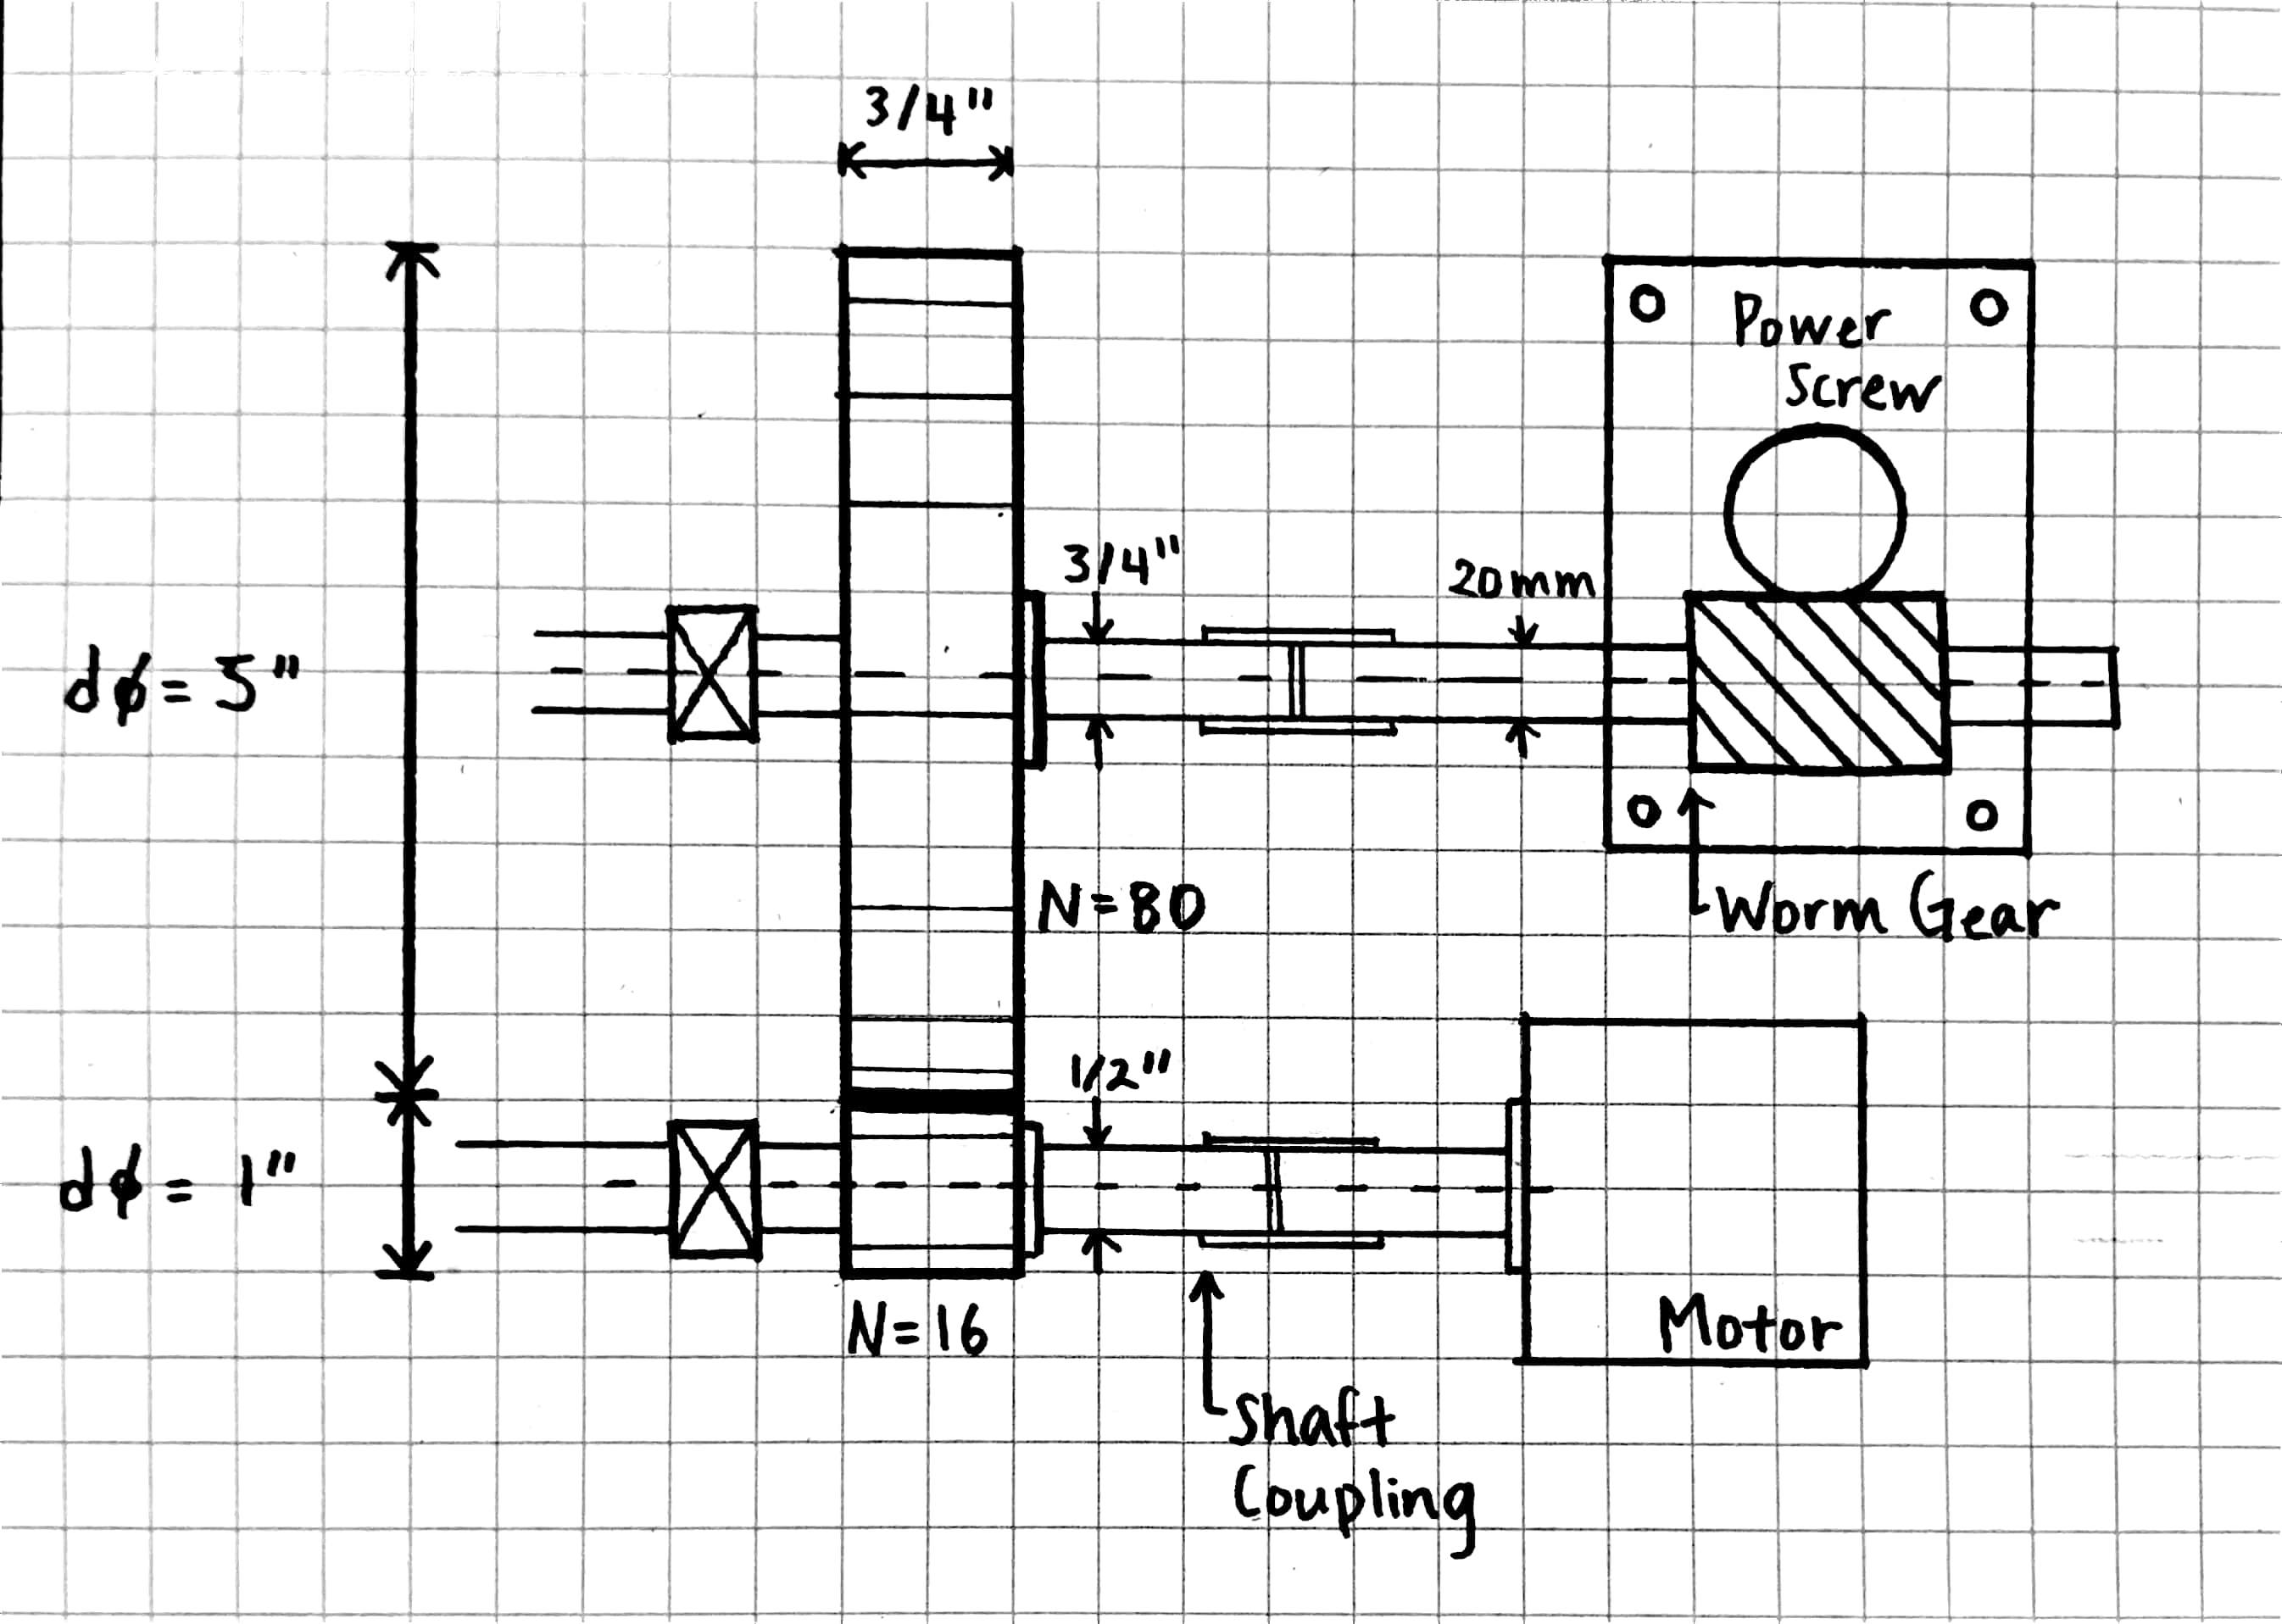
\includegraphics[width=16cm]{MECH325A1System}
\end{center}

\subsection{Optimization Script}
To find the most optimal outcome regarding the proposed performance metric, our team decided to create a script which will loop through all permutations of gear combinations and calculate the performance metric for each pair of pinion and gear. The script can be found at the GitHub repository below: \\
\begin{center}
    https://github.com/DonneyF/MECH-325-Assignments
\end{center}

\newpage

\section{Appendix}

\subsection{Power Screw Analysis}

The objective of this section is to verify the power screw is self-locking and find the minimum required torque and rotational speed needed to lift the 2500 kg load at 4 mm/sec.
Self-locking is ensured when the coefficient of thread friction is greater than a threshold defined as follows:
\begin{equation}
f > \tan(\lambda)
\end{equation}
$$\tan\lambda = \frac{l}{\pi d_m} = 0.0335$$
Since $f = 0.08 > \tan\lambda = 0.03$, the current design is self-locking. \\
\\
The torque required to lift the given load with gravitational force $F$ is:

\begin{equation}
\tau_{raise} = \frac{Fd_m}{2}\left(\frac{l+\pi f d_m}{\pi d_m - fl}\right)
\end{equation}
\\
The torque required to lower the given load with gravitational force $F$ is:

\begin{equation}
\tau_{lower} = \frac{Fd_m}{2}\left(\frac{\pi f d_m-l}{\pi d_m + fl}\right)
\end{equation}


\begin{center}
	\begin{tabular}{ |p{2cm}||p{3cm}|p{2cm}|p{7cm}|  }
		\hline
		\multicolumn{4}{|c|}{Parameters} \\
		\hline
		Symbol& Value & Units & Description\\
		\hline
		$F$ & $2500 \times 9.81$ & N & Axial compressive force\\
        $d$ & 60 & mm   & Major diameter\\			
		$d_m$ & 57 & mm   & Mean diameter, $d - \frac{l}{2}$\\
		$l$ & 6 & mm &  Pitch\\
		$f$ & 0.08 & N/A & Friction Coefficient\\
		\hline
	\end{tabular}
\end{center}

A torque of 79.5 Nm is required to lift the load and 32.4 Nm is required to lower the load, where efficiency losses in the power screw is accounted for by the friction coefficient, $f$. 
    
\subsection{Worm Gear Analysis}
Worm gears are used in high torque applications but they are subject to efficiency losses during operation. Calculating this value allows us to find the gear train required to raise the load. \\

	\begin{equation}
	\eta = \frac{\cos\phi_n - f\tan\lambda}{\cos\phi_n+f\cot\lambda}
	\end{equation}
\\	
The lead angle component is as follows:
	\begin{equation}
\tan \lambda =  \frac{p_x}{\pi d_p} = 0.4074366
	\end{equation}
We find the worm gear is therefore $80.34 \% $ efficient.
\begin{center}
		\begin{tabular}{ |p{2cm}||p{3cm}|p{2cm}|p{7cm}|  }
			\hline
			\multicolumn{4}{|c|}{Parameters} \\
			\hline
			Symbol& Value & Units & Description\\
			\hline
			$N_G$ & $18$ & N/A & Number of teeth on worm drive gear\\
			$N_w$ & 2 & N/A   & 2-thread worm \\
			$\phi_n$ & 14.5 & degrees &  Pressure angle\\
			$l$ & 16 & mm & pitch\\
			$p_x$ & 32 & mm & Axial pitch\\
			$d_p$ & 25 & mm & Worm pitch diameter\\
			$d_s$ & 20 & mm & Worm shaft diameter\\
			\hline
		\end{tabular}
	\end{center}
The 2-threaded worm gear engages with an 18 teeth worm drive nut. For each 9 revolution of the worm gear, the nut completes 1 revolution, resulting in a 9 fold torque increase. 

$$\frac{\tau }{9 \eta_{\text{worm}}} = \frac{79.5}{9(0.8034)} = 11.0 \text{ Nm}$$
\\
Therefore, the system requires 11.0 Nm to reach the worm gear. 

\subsection{Motor Torque and Gear Reduction}
The motor provided has the following torque-speed curve. The maximum power output occurs when the motor operates at 2500 rpm with 2.5 Nm of torque. \\

\begin{figure}[htbp] 
    \centering 
\begin{tikzpicture}
\begin{axis}[
    xmin = 0, xmax = 5000,
     ymin = 0, ymax = 7,    
    axis y line*=left,
    xlabel = Speed (RPM),
    ylabel = {Torque (Nm)},
    xtick={0,2000,4000},
    ytick = {0,1,2,3,4,5,6,7},
    legend pos = outer north east
]

\addplot [
    domain=0:5000, 
    samples=100, 
    color=blue,
    ]
    {-x/1000.0+5};
\end{axis}

   \begin{axis}[
     xmin = 0, xmax = 5000,
     ymin = 0, ymax = 700,
     hide x axis,
     hide y axis]
     \addplot [
    domain=0:5000, 
    samples=100, 
    color=red,
]
{(-x/1000.0+5)*(x*2*3.1415926/60.0)};
   \end{axis}
   \pgfplotsset{every axis y label/.append style={rotate=180,yshift=9.5cm}}
   \begin{axis}[
         xmin=0, xmax=5000,
         ymin=0, ymax=700,
         hide x axis,
         axis y line*=right,
         ylabel={Power (W)}
     ]
   \end{axis}
\end{tikzpicture}
\caption{Torque and power curve for chosen motor. Blue shows the torque and red shows the power output. Power is maximized at 2500 RPM.}
\end{figure}
\noindent The relationship to determine train value given torque specifications, $e$ is:
\begin{equation}
e = \frac{T_{\text{in}}f_{g}}{T_{\text{out}}} = \frac{2.5}{11} f_{g} = 0.227f_g
\end{equation}
where $T_{out}$ = torque output, $T_{in}$ = torque input, and $f_g$ = gear efficiency. \\
Spur gears are selected for their efficiency, between 94 - 98 \%, and simplicity. We assume the lower bound of efficiency. 
\begin{eqnarray}
\text{(simple two-gear system)}    \indent\indent &e = (0.227)(0.94) = 0.2136\\
\text{(compound four-gear system)} \indent\indent &e = (0.227)(0.94)^2 = 0.2 
\end{eqnarray}

\noindent If only two gears are used, select gear ratio to be at least 1:4.68. If a compound four gear system is appropriate, select gear ratio to be at least 1: 5.0.

\subsection{Motor Speed Calculation}
The raising and lowering torques for the load are used to compute torque at the motor which in turn gives the motor revolution per minute (rpm) as seen in figure 1. 
$$\tau_{\text{motor, raise}} = 79.5 (e)(\text{worm-power screw ratio}) \ (0.94*0.8034) = 2.34 Nm$$
$$\tau_{\text{motor, lower}} = 32.41 (e)(\text{worm-power screw ratio}) \ (0.94*0.8034) = 0.95 Nm$$
The worm-power screw ratio is 1/9. From the motor torque-speed curve, $\text{torque} = -\text{speed}/1000.0+5$, the raising rpm is 2659 and lowering rpm is 4050 rpm. 

\subsection{Power screw Speed Calculation}
The raising and lowering speed of power screw is dependent on motor rpm. 

\subsection{Bending \& Contact Stress Analysis}

Detailed stress analysis was performed on each gear and pinion considered for the design of the gear train. Major stress factors were determined to come from the bending and contact stresses exerted on the gear/pinion system during meshing. The following equation was used calculate and verify the allowable bending stress:

\begin{equation}
\sigma_{bending} = W^t K_o K_v K_s \frac{P_d}{F}\frac{K_s K_B}{J} \\
\end{equation}

\begin{center}
	\begin{tabular}{ |p{2cm}||p{2cm}|p{2.3cm}|p{2.3cm}|p{6cm}|  }
		\hline
		\multicolumn{5}{|c|}{Parameters} \\
		\hline
		Symbol & Units & Gear Values & Pinion Values & Description\\
		\hline
		$W^t$ & lbf & 41.612 & 41.612 & Tangential transmitted load\\
		$K_o$ & N/A & 1.75 & 1.75 & Overload factor\\
		$K_v$ & N/A & 1.433 & 1.433 & Dynamic factor\\
		$K_s$ & N/A & 0.980 & 0.980 & Size factor\\
		$P_{d}$ & 1/in & 16 & 16 & Transverse diametral pitch\\
		$F$ & in & 0.75 & 0.75 & Face Width of narrower member\\
		$K_m$ & N/A & 1.188 & 1.188 & Load-distribution factor\\
		$K_{B}$ & N/A & 1 & 1 & Rim-thickness factor\\
		$J$ & N/A & 0.42 & 0.27 & Geometry factor (bending strength)\\
		\hline
	\end{tabular}
\end{center}

\noindent The contact stress measurement was taken into account by the following equation, along with the following new parameters:

\begin{equation}
\sigma_{contact} = C_{p}\sqrt{W^t K_o K_v K_s \frac{K_m}{d_P F}\frac{C_f}{I}}
\end{equation}

\begin{center}
	\begin{tabular}{ |p{2cm}||p{2cm}|p{2.3cm}|p{2.3cm}|p{6cm}|  }
		\hline
		\multicolumn{5}{|c|}{Parameters} \\
		\hline
		Symbol & Units & Gear Values & Pinion Values & Description\\
		\hline
		$C_p$ & $\sqrt{lbf/in^2}$ & 2290.604 & 2290.604 & Elastic Coefficient\\
		$C_f$ & N/A & 1 & 1 & Surface condition factor\\
		$d_P$ & in & 5 & 1 & Pitch diameter\\
		$I$ & N/A & 0.133 & 0.133 & Geometry Factor (pitting resistance)\\
		\hline
	\end{tabular}
\end{center}

\noindent From our analysis, we obtain the following: 

\begin{align*}
    \sigma_{b_{\text{gear}}} &= 4454.54 \text{ lbf/in$^2$} \\
    \sigma_{c_{\text{gear}}} &= 30270.38 \text{ lbf/in$^2$} \\
    \sigma_{b_{\text{pinion}}} &= 6857.85 \text{ lbf/in$^2$} \\
    \sigma_{c_{\text{pinion}}} &= 67336.92 \text{ lbf/in$^2$} 
\end{align*}

\noindent\textbf{Note:} Many of the factors are constants that were obtained from reading values off graphs and tables. Other values depend on the material, geometry, and physical properties of the gear and pinion. Furthermore, all the parameters in the stress equations are in U.S. customary units. \\

\noindent Here we will discuss the relevant formulas, equations, and references utilized to obtain parameter values found in the bending and contact stress equations. Note that all references to table and figure numbers are from Shigley's Mechanical Engineering Design Textbook.
\begin{itemize}[leftmargin=3mm]
    \item \textbf{2.4.1. Transmitted Load ($W^t$):} this parameter represents the load transmitted onto the teeth of the gear and pinion during their interaction. The transmitted load is calculated by finding the motor torque exerted on the pinion, finding the pitch diameter of the pinion, and then applying torque analysis, namely $T = Fr$ to find the transmitted force.
    
    \item \textbf{2.4.2. Bending-Strength Geometry Factor ($J$):} this factor is used to determine the bending strength of the spur gear teeth. Values for $J$ were directly read off of Figure 14-6 in Shigley's, and were determined based on the number of teeth on the gear and pinion.
    
    \item \textbf{2.4.3. Surface-Strength Geometry Factor ($I$):} this factor is used to determine the pitting resistance of the spur gear teeth. The surface-strength geometry factor is defined as follows:
    \begin{equation}
        I = \dfrac{\cos\phi_t \sin\phi_t}{2m_N} \dfrac{m_G}{m_G + 1}
    \end{equation}
    Where $\phi_t$ is the transverse pressure angle, $m_N$ is the load sharing ratio (1 for spur gears), and $m_G$ is the gear ratio.
    
    \item \textbf{2.4.4. Elastic Coefficient ($C_f$):} this factor is used to represent elastic properties of the pinion and gear during teeth interaction and meshing. The elastic coefficient is defined as follows:
    
    \begin{equation}
        C_p = \left[\dfrac{1}{\pi \left(\dfrac{1-v_P^2}{E_P} + \dfrac{1 - v_G^2}{E_G}\right)}\right]^2
    \end{equation}
    
    Where $v_P$, $v_G$ are the Poisson's ratio of the pinion and gear respectively, and $E_P$ and $E_G$ are the Modulus of Elasticity of the pinion and gear respectively. Based on Table 14-8 in Shigley's, the Poisson's ratio of the pinion and gear were determined to be at 0.30, and since the material for the pinion of gear is steel, the Modulus of Elasticity is $30 \times 10^6$ $\text{lbf/in}^2$ for both. 
    
    \item \textbf{2.4.5. Dynamic Factor ($K_v$):} this factor is used to account for inaccuracies in the manufacture and meshing of gear teeth in action. The dynamic factor is defined as follows:
    \begin{equation}
        K_v = \left(\dfrac{A + \sqrt{V}}{A}\right)^B
    \end{equation}
    Where the constants are defined as:
    \begin{align*}
        A &= 50 + 56(1-B) \\
        B &= 0.25(12-Q_v)^{2/3}
    \end{align*}
    Where $Q_v$ is the AGMA transmission accuracy number. For our analysis, we decided to use a $Q_v$ value of 5 since 3-7 is the range for commercial use.
    
    \item \textbf{2.4.6. Overload Factor ($K_o$):} this factor is used to make allowance for all externally applied loads in excess of the nominal tangential load $W^t$. The value for $K_o$ was determined using Figures 14-17 and 14-18, from which a value of 1.75 was obtained since we are assuming there will be an initial shock with uniform motion for the raising and lowering of the power screw system.
    
    \item \textbf{2.4.7. Surface Condition Factor ($C_f$):} this factor is used to represent any defects in the gear surface, which could have been caused by residual stress, poor surface finishing, or plastic effects. Since we assume the new gears and pinions purchased to be in good condition, we assign a value of 1 to $C_f$.
    
    \item \textbf{2.4.8. Size Factor ($K_s$):} this factor reflects the non-uniformity of material properties due to size. The size factor is defined as follows:
    \begin{equation}
        K_s = 1.192 \left(\dfrac{F \sqrt{Y}}{P}\right)^{0.0535}
    \end{equation}
    Where $F$ is the face width of the narrowest member, $Y$ is the Lewis Form Factor of the gear/pinion, and $P$ is the diametral pitch. Values for $Y$ was determined using Table 14-2.
    
    \item \textbf{2.4.9. Load-Distribution Factor ($K_m$):} this factor reflects nonuniform distribution of load across the line of contact. The load-distribution factor is defined as follows:
    \begin{equation}
        K_m = 1 + C_{mc}(C_{pf}C_{pm} + C_{ma}C_{e})
    \end{equation}
    Where $C_{mc} = 1$ since we are using gears/pinions with uncrowned teeth, $C_{pm} = 1$ since the ratio between then pinion offset from center span, $S_1$, and bearing span, $S$, is less than 0.175, and $C_e = 1$ since our pinions/gears are not adjusted at assembly. \\\\
    $C_{pf}$ is defined as follows: 
    \begin{equation}
    C_{pf} = \begin{cases} 
	\frac{F}{10d} - 0.025 & F \leq 1 \text{ in} \\
	\frac{F}{10d} -0.0375+0.0125F & 1 < F \leq 17 \text{ in}
	\end{cases} 
	\end{equation}
    Where $F$ is the minimum face width of the narrowest member and $d$ is the pitch diameter. \\\\
    Next, we calculate $C_{ma}$ as follows:
    \begin{equation*}
        C_{ma} = A + BF + CF^2
    \end{equation*}
    Where $A$, $B$, and $C$ are constants obtained from Table 14-9. We decided to use commercial-grade conditioning for our gears/pinions, and set $A$ = 0.127, $B$ = 0.0158, and $C$ = -0.930($10^{-4}$).
    
    \item \textbf{2.4.10. Rim-Thickness Factor ($K_B$):} this factor represents is the ratio of rim thickness $t_R$ and tooth height $h_t$. We downloaded the CAD model and measured the respective distances to obtain the backup ratio: 
    \begin{equation*}
    m_B = \frac{t_R}{h_t}
    \end{equation*}
    We obtain the following:
    \begin{equation*}
        m_{B_{\text{pinion}}} &= \frac{ 0.421875}{0.140625} = 3, \text{ }m_{B_{\text{gear}}} &= \frac{ 0.421875}{0.140625} = 9.5
    \end{equation*}
    Since all $m_B \geq 1.2$, $K_B = 1$.

\end{itemize}

\subsection{Safety Factor Analysis}
To ensure the gear train system maintains an acceptable level of safety (2.2 minimum), bending and contact safety factors were calculated to validate design specifications.

\begin{equation}
S_{F(bending)} = \frac{S_t}{\sigma_b}\frac{Y_N}{K_T K_R} \\
\end{equation}
\begin{equation}
S_{H(contact)} = \frac{S_c}{\sigma_c}\frac{Z_N C_H}{K_T K_R}
\end{equation}

\begin{center}
	\begin{tabular}{ |p{2cm}||p{2cm}|p{2.3cm}|p{2.3cm}|p{6cm}|  }
		\hline
		\multicolumn{5}{|c|}{Parameters} \\
		\hline
		Symbol & Units & Gear Values & Pinion Values & Description\\
		\hline
		$S_t$ & bf/in$^2$ & 32125 & 32125 & AGMA bending strength\\
		$S_c$ & lbf/in$^2$ & 109600 & 109600 & AGMA surface endurance strength\\
		$Y_N$ & N/A & 1.890 & 1.890 & Stress cycle (bending strength)\\
		$Z_N$ & N/A & 1.42 & 1.42 & Stress cycle (pitting resistance)\\
		$C_H$ & N/A & 1 & 1 & Hardness-ratio factor\\
		$\sigma_b$ & lbf/in$^2$ & 4454.54 & 6857.85 & Bending stress\\
		$\sigma_c$ & lbf/in$^2$ & 30270.38 & 67336.92 & Contact stress\\
		$K_T$ & N/A & 1 & 1 & Temperature factor\\
		$K_R$ & N/A & 0.955 & 0.955 & Reliability factor\\
		\hline
	\end{tabular}
\end{center}

\noindent From our analysis, we obtain the following: 

\begin{align*}
    S_F_{\text{gear}} &= 14.27 \\
    S_H_{\text{gear}} &= 5.37 \\
    S_F_{\text{pinion}} &= 9.27 \\
    S_H_{\text{pinion}} &= 2.414
\end{align*}

\noindent Here we will discuss the relevant formulas, equations, and references utilized to obtain parameter values found in the safety factor equations. Note that all references to table and figure numbers are from Shigley's Mechanical Engineering Design Textbook.
\begin{itemize}[leftmargin=3mm]
    \item \textbf{2.5.1. Allowable Bending/Contact Stress Number ($S_t$, $S_c$):} this parameter represents AGMA defined stress numbers, obtained from Figures 14-2 and 14-5. Since we are using Grade 1 steel gears/pinions, we are able to calculate the stress numbers using the following:
    \begin{align*}
        S_t &= 77.3\text{ }H_B + 12800 \text{ psi} \\
        S_c &= 322\text{ }H_B + 29100 \text{ psi}
    \end{align*}
    Where $H_B$ is the Brinell Hardness of the steel gears/pinions.
    
    \item \textbf{2.5.2. Stress-Cycle Factors} ($Y_N$ and $Z_N$): this factor reflects the number of load cycles the gear/pinion can sustain through. From Figures 14-14 and 14-15, we can calculate $Y_N$ and $Z_N$ by the following:
    \begin{align*}
        Y_N &= 6.1514 N^{-0.1192} \\
        Z_N &= 2.466 N^{-0.056}
    \end{align*}
    Where N is the number of load cycles, which is a minimum of $2 \times 10^4$ in this case.
    
    \item \textbf{2.5.3. Hardness-Ratio Factor ($C_H$):} this factor is used to account for the effect obtained when a surface-hardened pinion is mated with a through-hardened gear, and adjust the surface strengths for this effect. The hardness-ratio factor is defined as follows:
    \begin{equation}
        C_H = 1.0 + A'(m_G = 1.0)
    \end{equation}
    Where:
    \begin{equation*}
        A' = 8.98(10^{-3})\left(\dfrac{H_{BP}}{H_{BG}}\right) - 8.29(10^{-3})\text{ }1.2 \leq \frac{H_{BP}}{H_{BG}} \leq 1.7
    \end{equation*}
    From which we note that:
    \begin{align*}
        \dfrac{H_{BP}}{H_{BG}} &< 1.2, \text{ $A' = 0$} \\
        \dfrac{H_{BP}}{H_{BG}} &> 1.7, \text{ $A' = 0.00698$}
    \end{align*}
    The terms $H_{BP}$ and $H_{BG}$ are the Brinell hardness of the pinion and gear, respectively. Since we are using steel material, the Brinell hardness of both the pinion and gear are 350 HB as described in the assignment document. \\\\
    Therefore, the ratio of Brinell hardness is less than 1, from which we obtain that $A' = 0$. Therefore, $C_H = 1$.
    
    \item \textbf{2.5.4. Reliability Factor ($K_R$):} this factor accounts for the effect of the statistical distributions of material fatigue failures. The reliability factor is defined as follows:
    \begin{equation}
    K_R = 0.658-0.0759\ln{(1-R)}
    \end{equation}
    Where $R$ is the reliability factor, out of 1. We determined that a safety factor of 0.98 would be sufficient for our gear system, and thus we obtain a $K_R$ value of 0.955.
    
    \item \textbf{2.5.5. Temperature Factor ($K_T$):} this factor reflects the limits of temperature values that can be used for proper stress analysis. Since we assume that our gears/pinions never reach a temperature value higher than or equal to $120^\circ$C during operation, $K_T$ = 1.
\end{itemize}

\subsection{Performance Metric Analysis}



\end{document}
